\documentclass[12pt]{article}

\usepackage[english]{babel}
\usepackage{blindtext}
\usepackage{graphicx}
\usepackage{amssymb}
\usepackage{amsthm}
\usepackage{amsmath}
\usepackage{bbold}
%\textsc{•}\usepackage{bm}
%\usepackage{physics}
\usepackage[a4paper, width = 185mm, top = 15mm, bottom = 15mm]{geometry}
\usepackage{calligra}
\usepackage{float}

\DeclareMathAlphabet{\mathcalligra}{T1}{calliga}{m}{n}
\DeclareFontShape{T1}{calligra}{m}{n}{<->s*[2.2]callig15}{}

\newcommand{\scripty}[1]{\ensuremath{\mathcalligra{#1}}}
\renewcommand* \d{\mathop{}\!\mathrm{d}}



\begin{document}
\noindent
The Hedin equations are given by:
\begin{align}
G(x_1,x_2)&=G^0(x_1,x_2)+\int \d x_3\d x_4 G^0(x_1,x_3)\Sigma(x_3,x_4)G(x_4,x_2)\\
\Sigma(x_1,x_2) &= i\int\d x_3\d x_4 \Gamma(x_4;x_1,x_3)G(x_3,x_2)W(x_4,x_2)\\
\Gamma(x_1;x_2,x_3)&=\delta(x_1-x_2)\delta(x_1-x_3)+\int \d x_4\d x_5\d x_6\d x_7 \Gamma(x_1;x_4,x_5)G(x_6,x_4)G(x_5,x_7)\dfrac{\delta\Sigma(x_2,x_3)}{\delta G(x_6,x_7)}\\
\Pi(x_1,x_2)&=-i\int \d x_3\d x_4\Gamma(x_1;x_3,x_4)G(x_2,x_3)G(x_4,x_2)\\
W(x_1,x_2)&=v(\vec{x}_1,\vec{x}_2)\delta(t_1-t_2)+\int \d x_3\d x_4v(\vec{x_1},\vec{x}_3)\delta(t_1-t_3)\Pi(x_3,x_4)W(x_4,x_2)
\end{align}
Where $x_1 = (\vec{x}_1, t_1)$. This closed set of equations can be represented by the following diagram:
\begin{figure}[h!]
\center
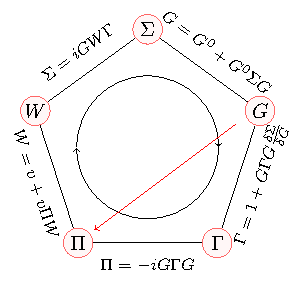
\includegraphics[scale=1.5]{images.pdf}
\end{figure}\\
For the GW approximation we start with a given $G^0$ and take $\Sigma=0$. One cycle through the diagram gives:
\begin{align}
G(x_1,x_2)&=G^0(x_1,x_2)\\
\Gamma(x_1;x_2,x_3)&=\delta(x_1-x_2)\delta(x_1-x_3)\\
\Pi(x_1,x_2)&=-i\int \d x_3\d x_4\delta(x_1-x_3)\delta(x_1-x_4)G^0(x_2,x_3)G^ 0(x_4,x_2)\\
&=-iG^0(x_2,x_1)G^0(x_1,x_2)\notag\\
W(x_1,x_2)&=v(\vec{x}_1,\vec{x}_2)\delta(t_1-t_2)+\int \d x_3\d x_4v(\vec{x_1},\vec{x}_3)\delta(t_1-t_3)\Pi(x_3,x_4)W(x_4,x_2)\\
\Sigma(x_1,x_2) &= i\int\d x_3\d x_4 \delta(x_4-x_1)\delta(x_4-x_3)G^0(x_3,x_2)W(x_4,x_2)\\
&= iG^0(x_1,x_2)W(x_1,x_2)\notag\\
G(x_1,x_2)&=G^0(x_1,x_2)+i\int \d x_3\d x_4 G^0(x_1,x_3)G^0(x_3,x_4)W(x_3,x_4)G(x_4,x_2)
\end{align}
\newpage
\noindent
We're currently in the time domain and want to Fourier transform to the frequency domain. Starting with a $G^0(\vec{x}_1,\vec{x}_2;\omega)$ we have:
\begin{align}
\Pi(\vec{x}_1,\vec{x}_2;\omega)=-i(G^0(\vec{x}_2,\vec{x}_1)*G^0(\vec{x}_1,\vec{x}_2))(\omega)=-i
\int\dfrac{\d \omega'}{2\pi}G^0(\vec{x}_2,\vec{x}_1; \omega - \omega' )G^0(\vec{x}_1,\vec{x}_2;\omega')
\end{align}
And
\begin{align}
W(\vec{x}_1,\vec{x}_2;\omega)&=\dfrac{1}{2\pi} v(\vec{x}_1,\vec{x}_2)+\mathcal{F}\bigg \{\int \d \vec{x}_3\d \vec{x}_4\d t_4v(\vec{x_1},\vec{x}_3)\Pi(x_1,x_4)W(x_4,x_2)\bigg \}\\
&=\dfrac{1}{2\pi} v(\vec{x}_1,\vec{x}_2)+\mathcal{F}\bigg \{\int \d \vec{x}_3\d \vec{x}_4\d t_4v(\vec{x_1},\vec{x}_3)\Pi(\vec{x}_1,\vec{x}_4;t_1-t_4)W(\vec{x}_4,\vec{x}_2; t_4-t_2)\bigg \}\notag\\
&=\dfrac{1}{2\pi} v(\vec{x}_1,\vec{x}_2)+\int \d \vec{x}_3\d \vec{x}_4v(\vec{x_1},\vec{x}_3)\mathcal{F}\bigg \{\int\d u\ \Pi(\vec{x}_1,\vec{x}_4;t-u)W(\vec{x}_4,\vec{x}_2; u)\bigg \}\notag\\
&=\dfrac{1}{2\pi} v(\vec{x}_1,\vec{x}_2)+\dfrac{1}{2\pi}\int \d \vec{x}_3\d \vec{x}_4v(\vec{x_1},\vec{x}_3)\Pi(\vec{x}_1,\vec{x}_4;\omega)W(\vec{x}_4,\vec{x}_2; \omega)\notag
\end{align}
And if the integrals are taken discreetly with $v$, $\Pi$ and $W$ matrices we'd get:
\begin{equation}
W(\omega)=(2\pi\mathbb{1}-v\Pi(\omega))^{-1}v
\end{equation}
For the self energy we get another convolution:
\begin{align*}
\Sigma(\vec{x}_1,\vec{x}_2;\omega)&=i\mathcal{F}\{G^0(\vec{x}_1,\vec{x}_2;t)W(\vec{x}_1,\vec{x}_2;t)\}=i\int\dfrac{\d \omega'}{2\pi}G^0(\vec{x}_1,\vec{x}_2; \omega - \omega' )W(\vec{x}_1,\vec{x}_2;\omega')
\end{align*}
And lastly the Green function can be obtained by inversion:
$$G(\vec{x}_1,\vec{x}_2,\omega)=[(G^0(\vec{x}_1,\vec{x}_2,\omega))^ {-1}-\Sigma(\vec{x}_1,\vec{x}_2,\omega)]^{-1}$$
Since convolutions in frequency space are product is temporal space we can avoid computing the convolutions and instead perform a Fourier transform and a product instead. This results in the following scheme:
\begin{figure}[h!]
\center
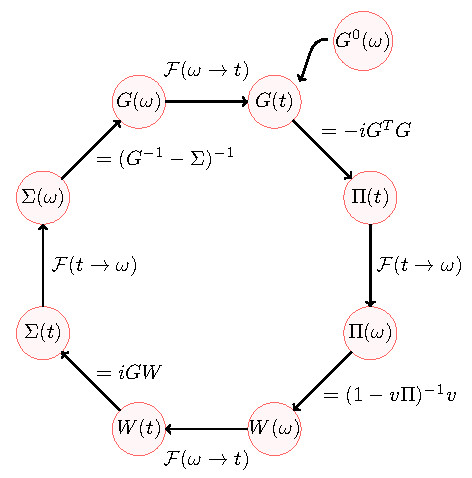
\includegraphics[scale=1.2]{images2.pdf}
\end{figure}\\
\newpage
\noindent
This scheme has been implemented using the TRIQS package. Below follow some results:
\begin{figure}[h!]
\center
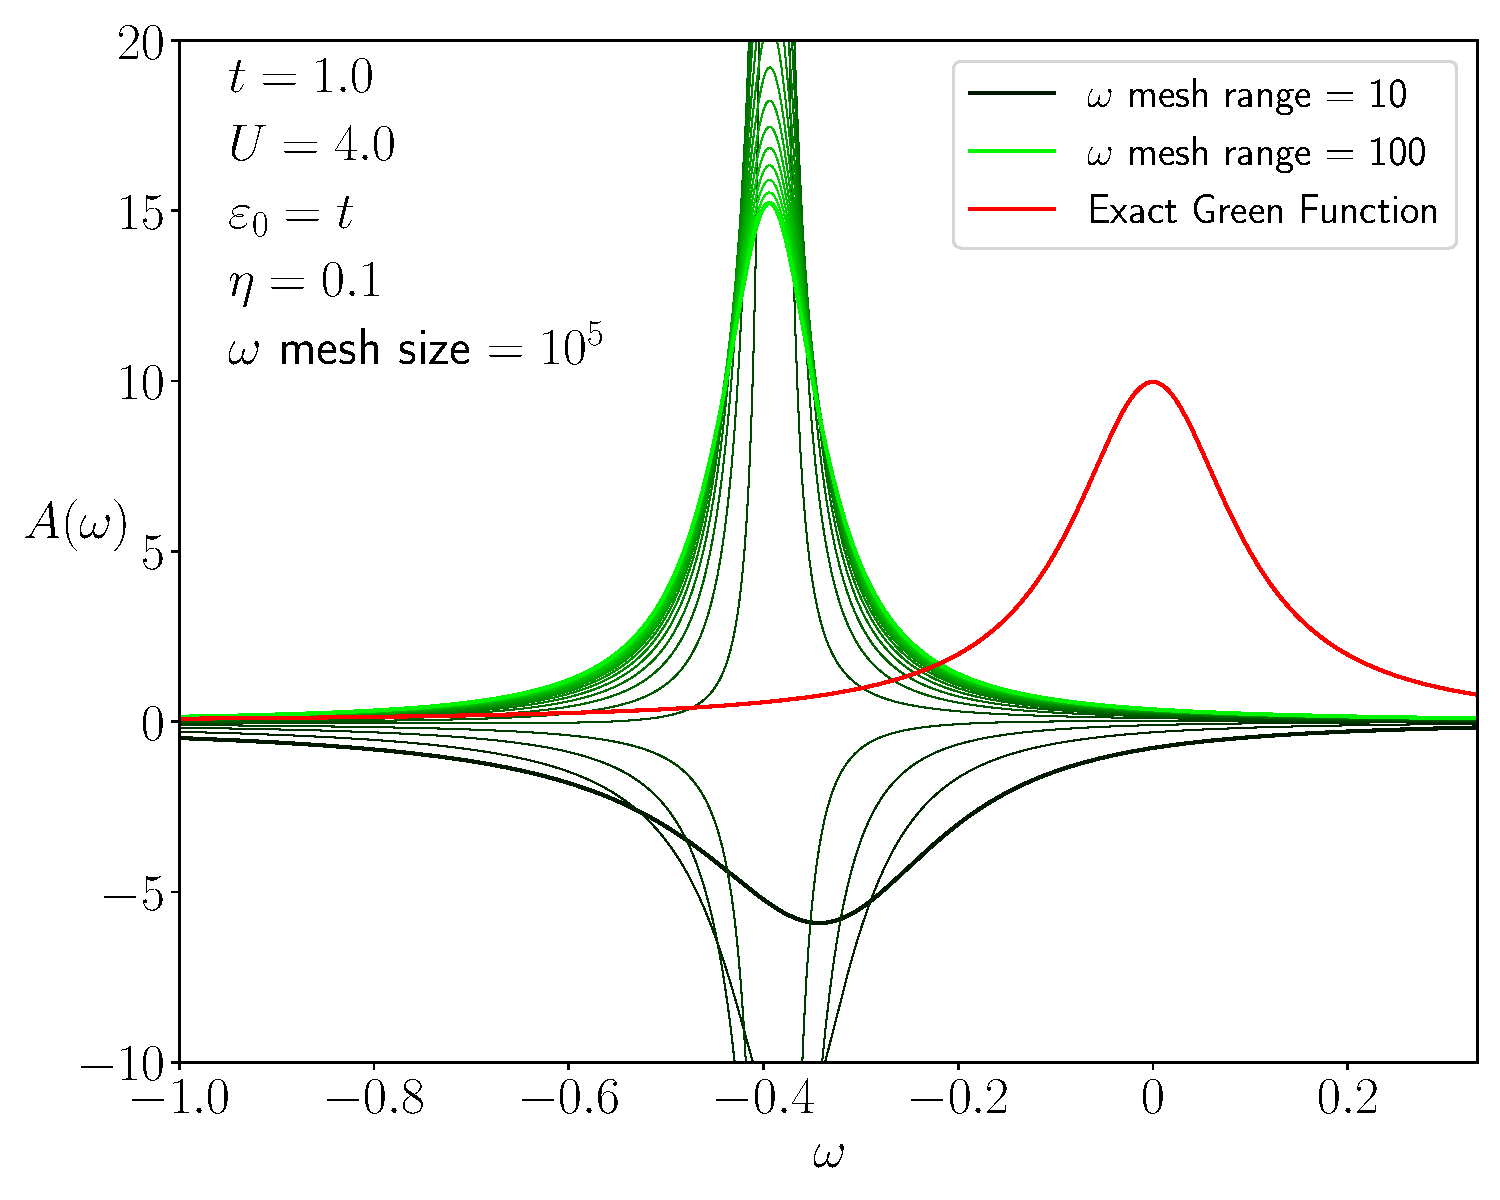
\includegraphics[scale=0.6]{wcomp.pdf}
\end{figure}
\begin{figure}[h!]
\center
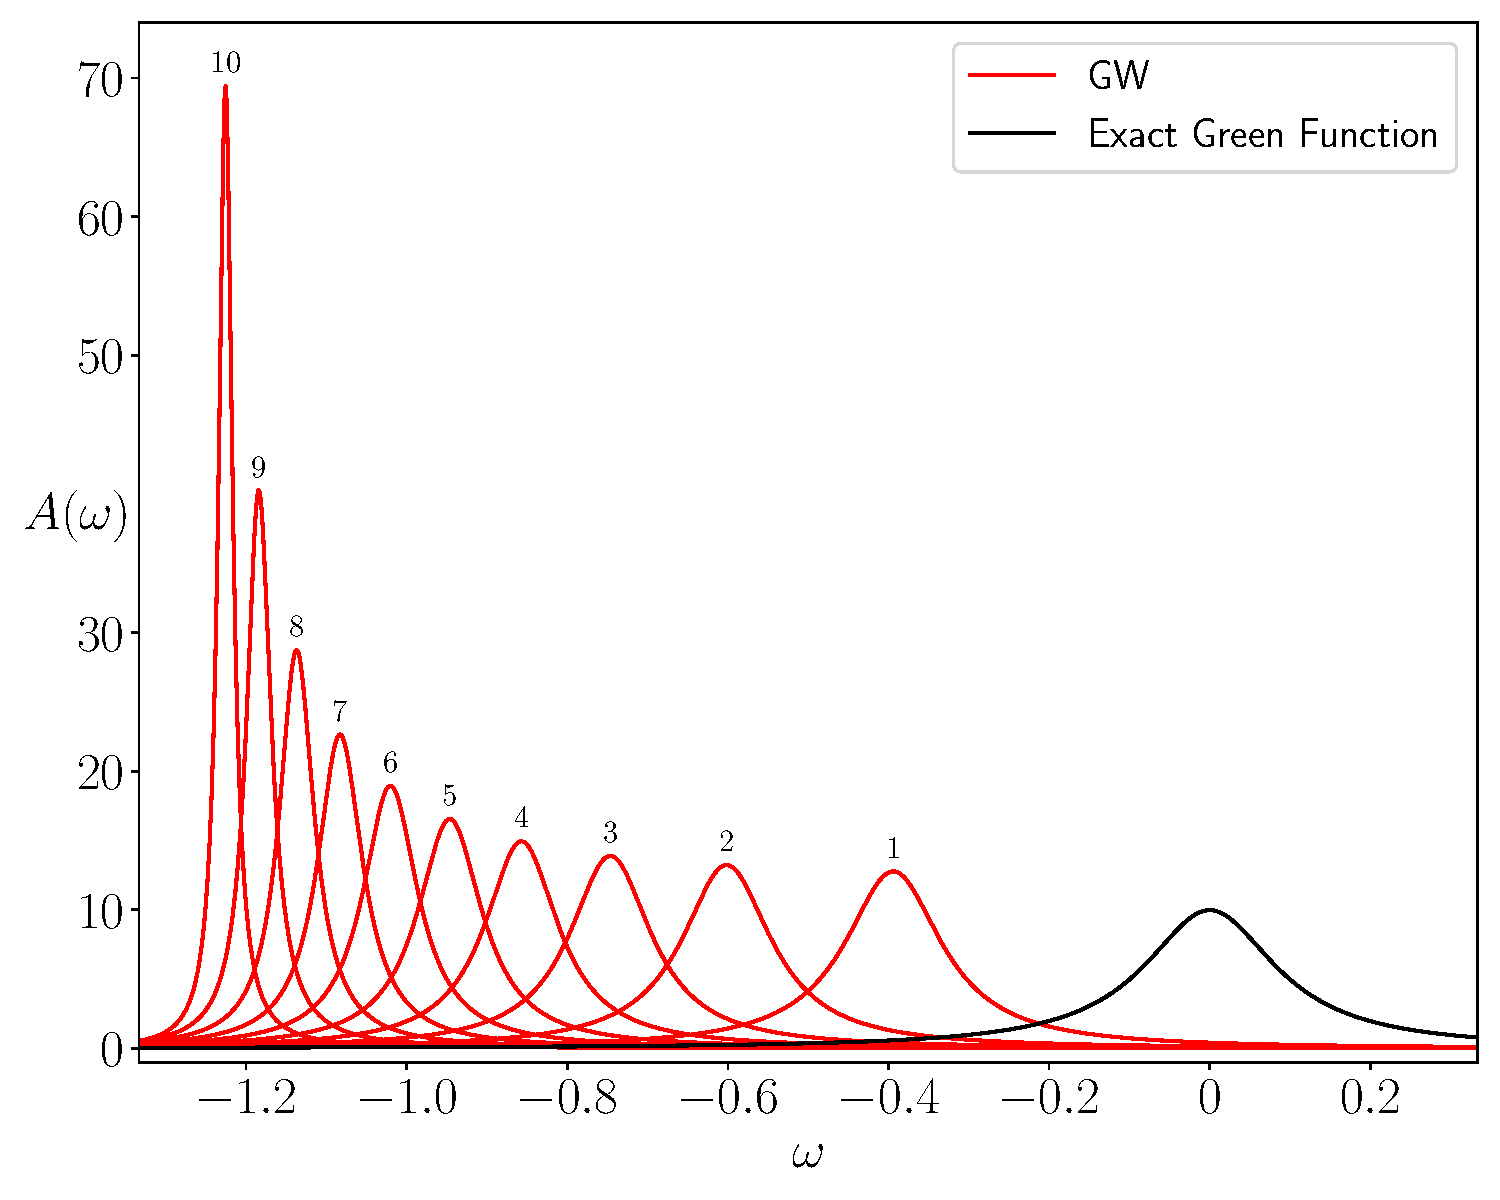
\includegraphics[scale=0.6]{ccomp.pdf}
\end{figure}\\

\begin{figure}[h!]
\center
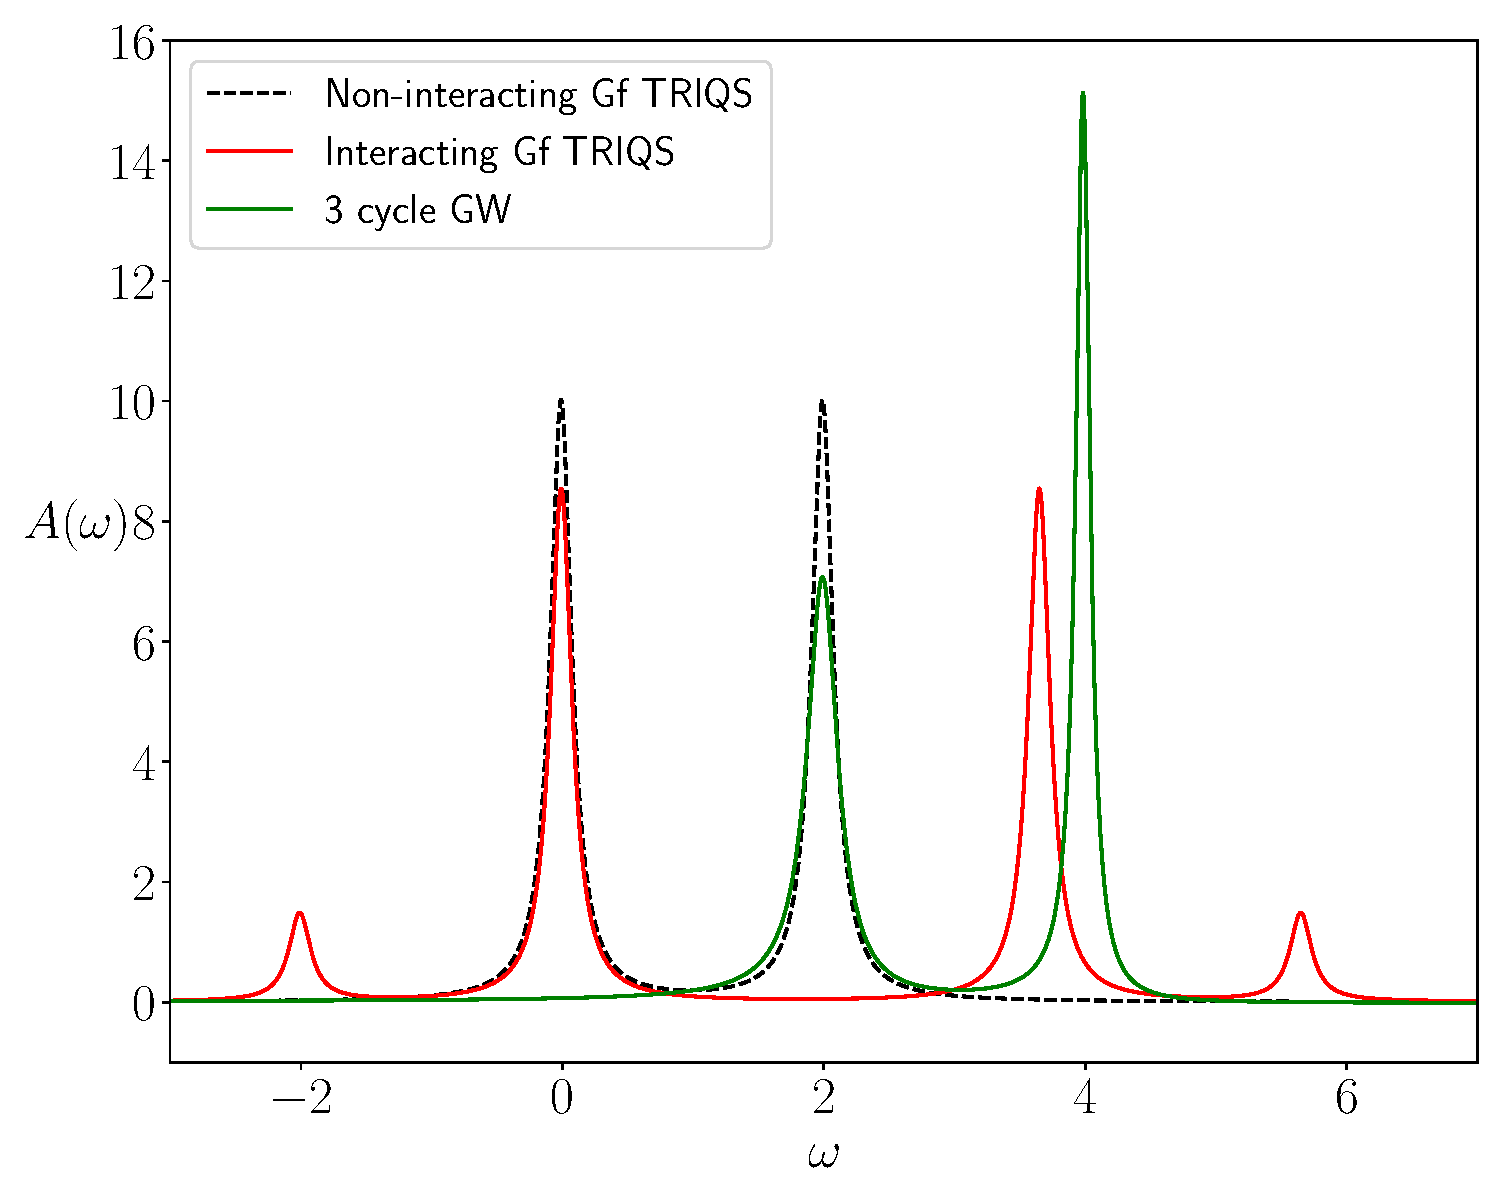
\includegraphics[scale=0.6]{qf.pdf}
\end{figure}
\begin{figure}[h!]
\center
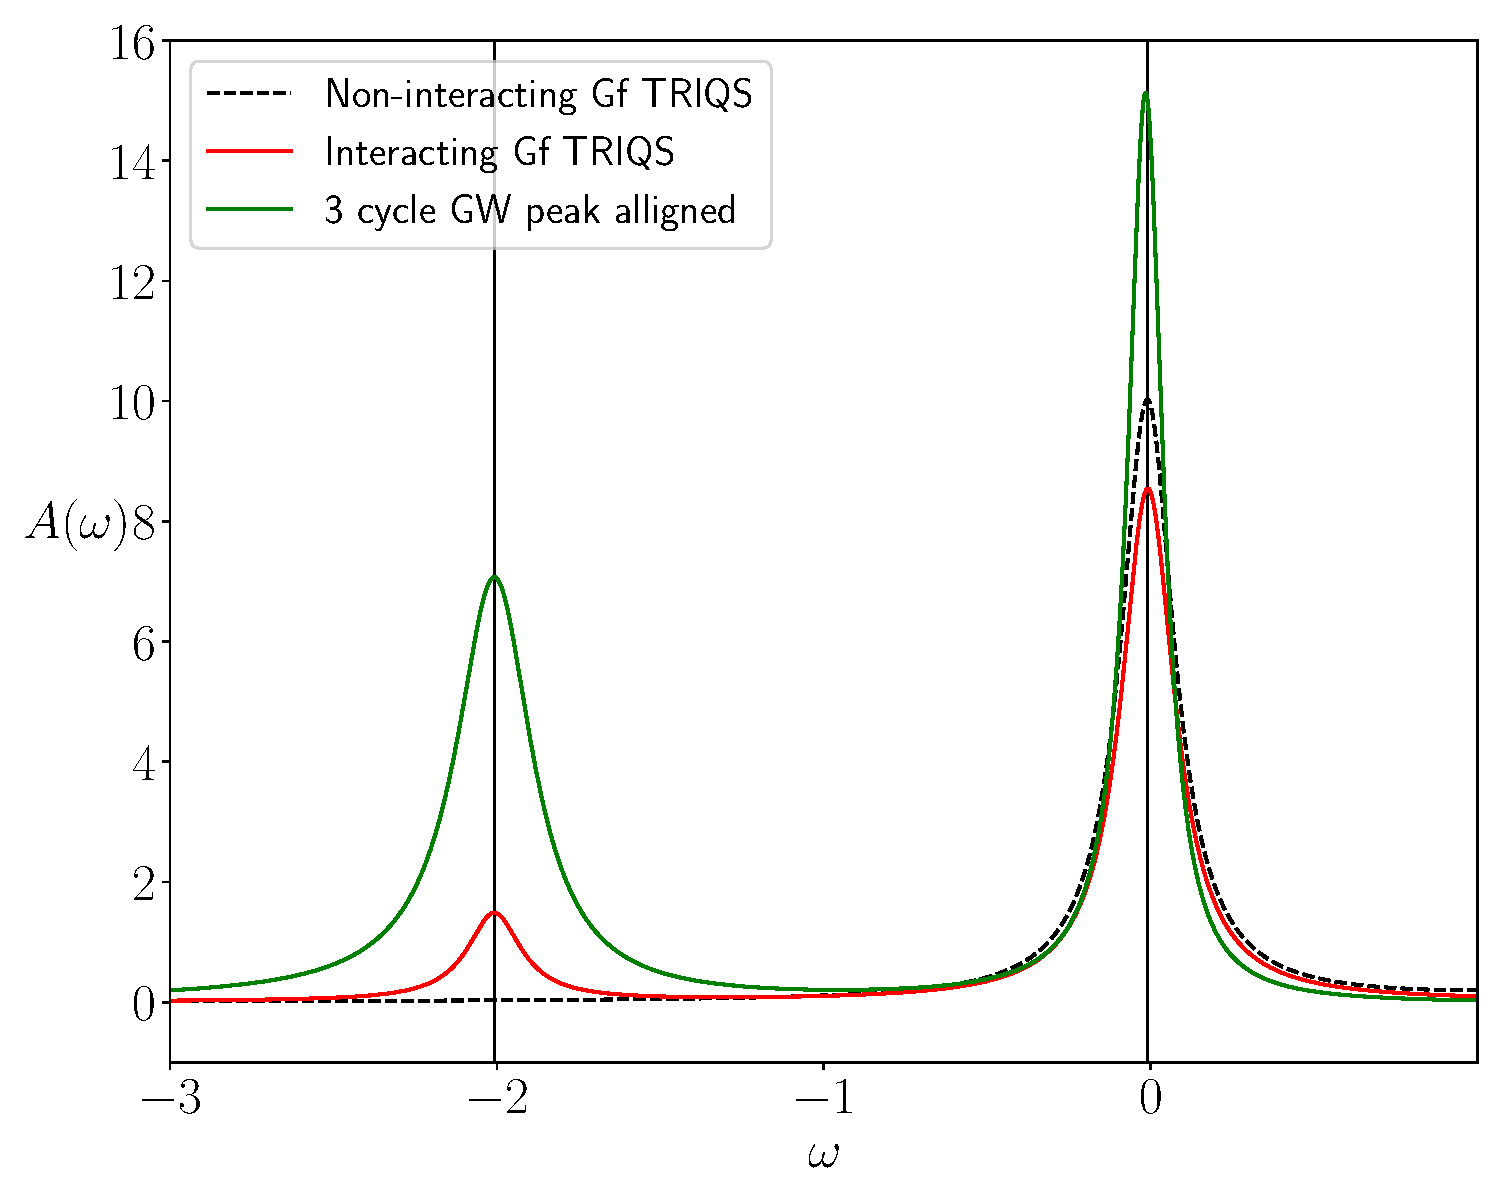
\includegraphics[scale=0.6]{aligned.pdf}
\end{figure}
\newpage
\noindent
When computing $G$ and $W$ we can either write it in this form:
\begin{align*}
G&=(1-G^0\Sigma)^{-1}G^0\\
W&=(1-v\Pi)^{-1}v
\end{align*}
Or instead as :
\begin{align*}
G&=({G^0}^{-1}-\Sigma)^{-1}\\
W&=(v^{-1}-\Pi)^{-1}
\end{align*}
I assume the double inversions in the second set of equations will be computationally heavier?
\newpage
\noindent
The code has been rewritten for Matsubara Green functions and has been applied to the Hubbard dimer at half-filling, just as Hugo Strand. We start with a non-interacting Green function obtained from the full Green function but setting $U=0$:

\begin{figure}[h!]
\center
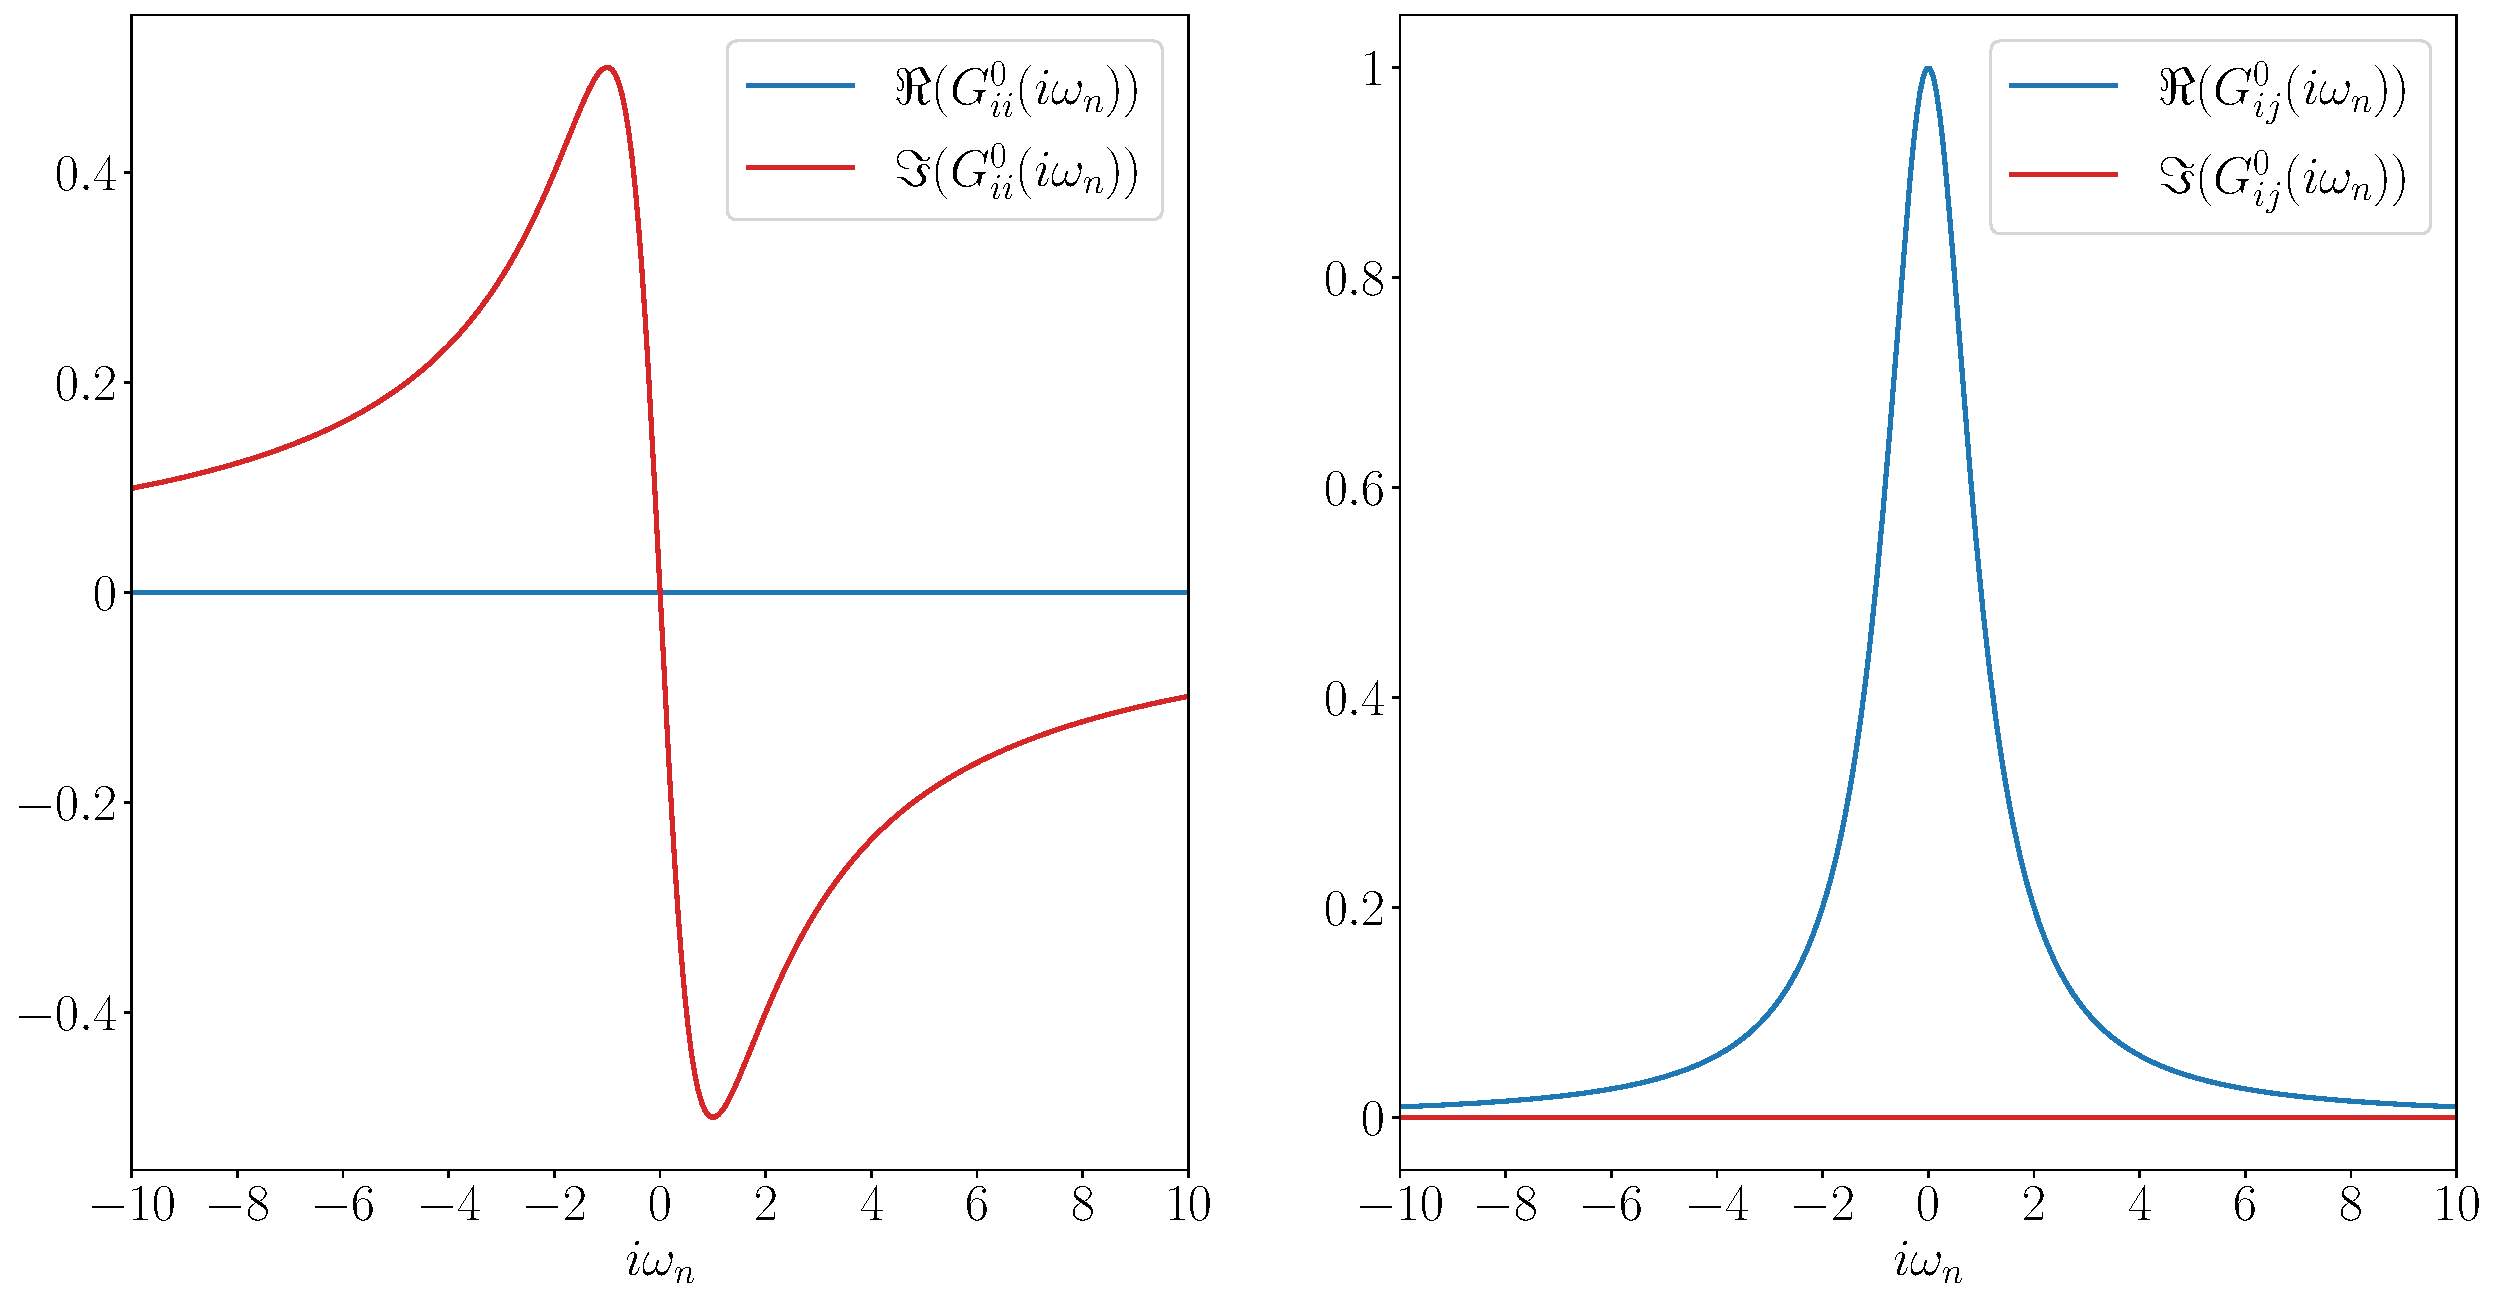
\includegraphics[scale=0.45]{G0.pdf}
\end{figure}
\begin{equation}
P(\tau)=-(G^0)^T(-\tau)G(\tau)	
\end{equation}
\begin{figure}[h!]
\center
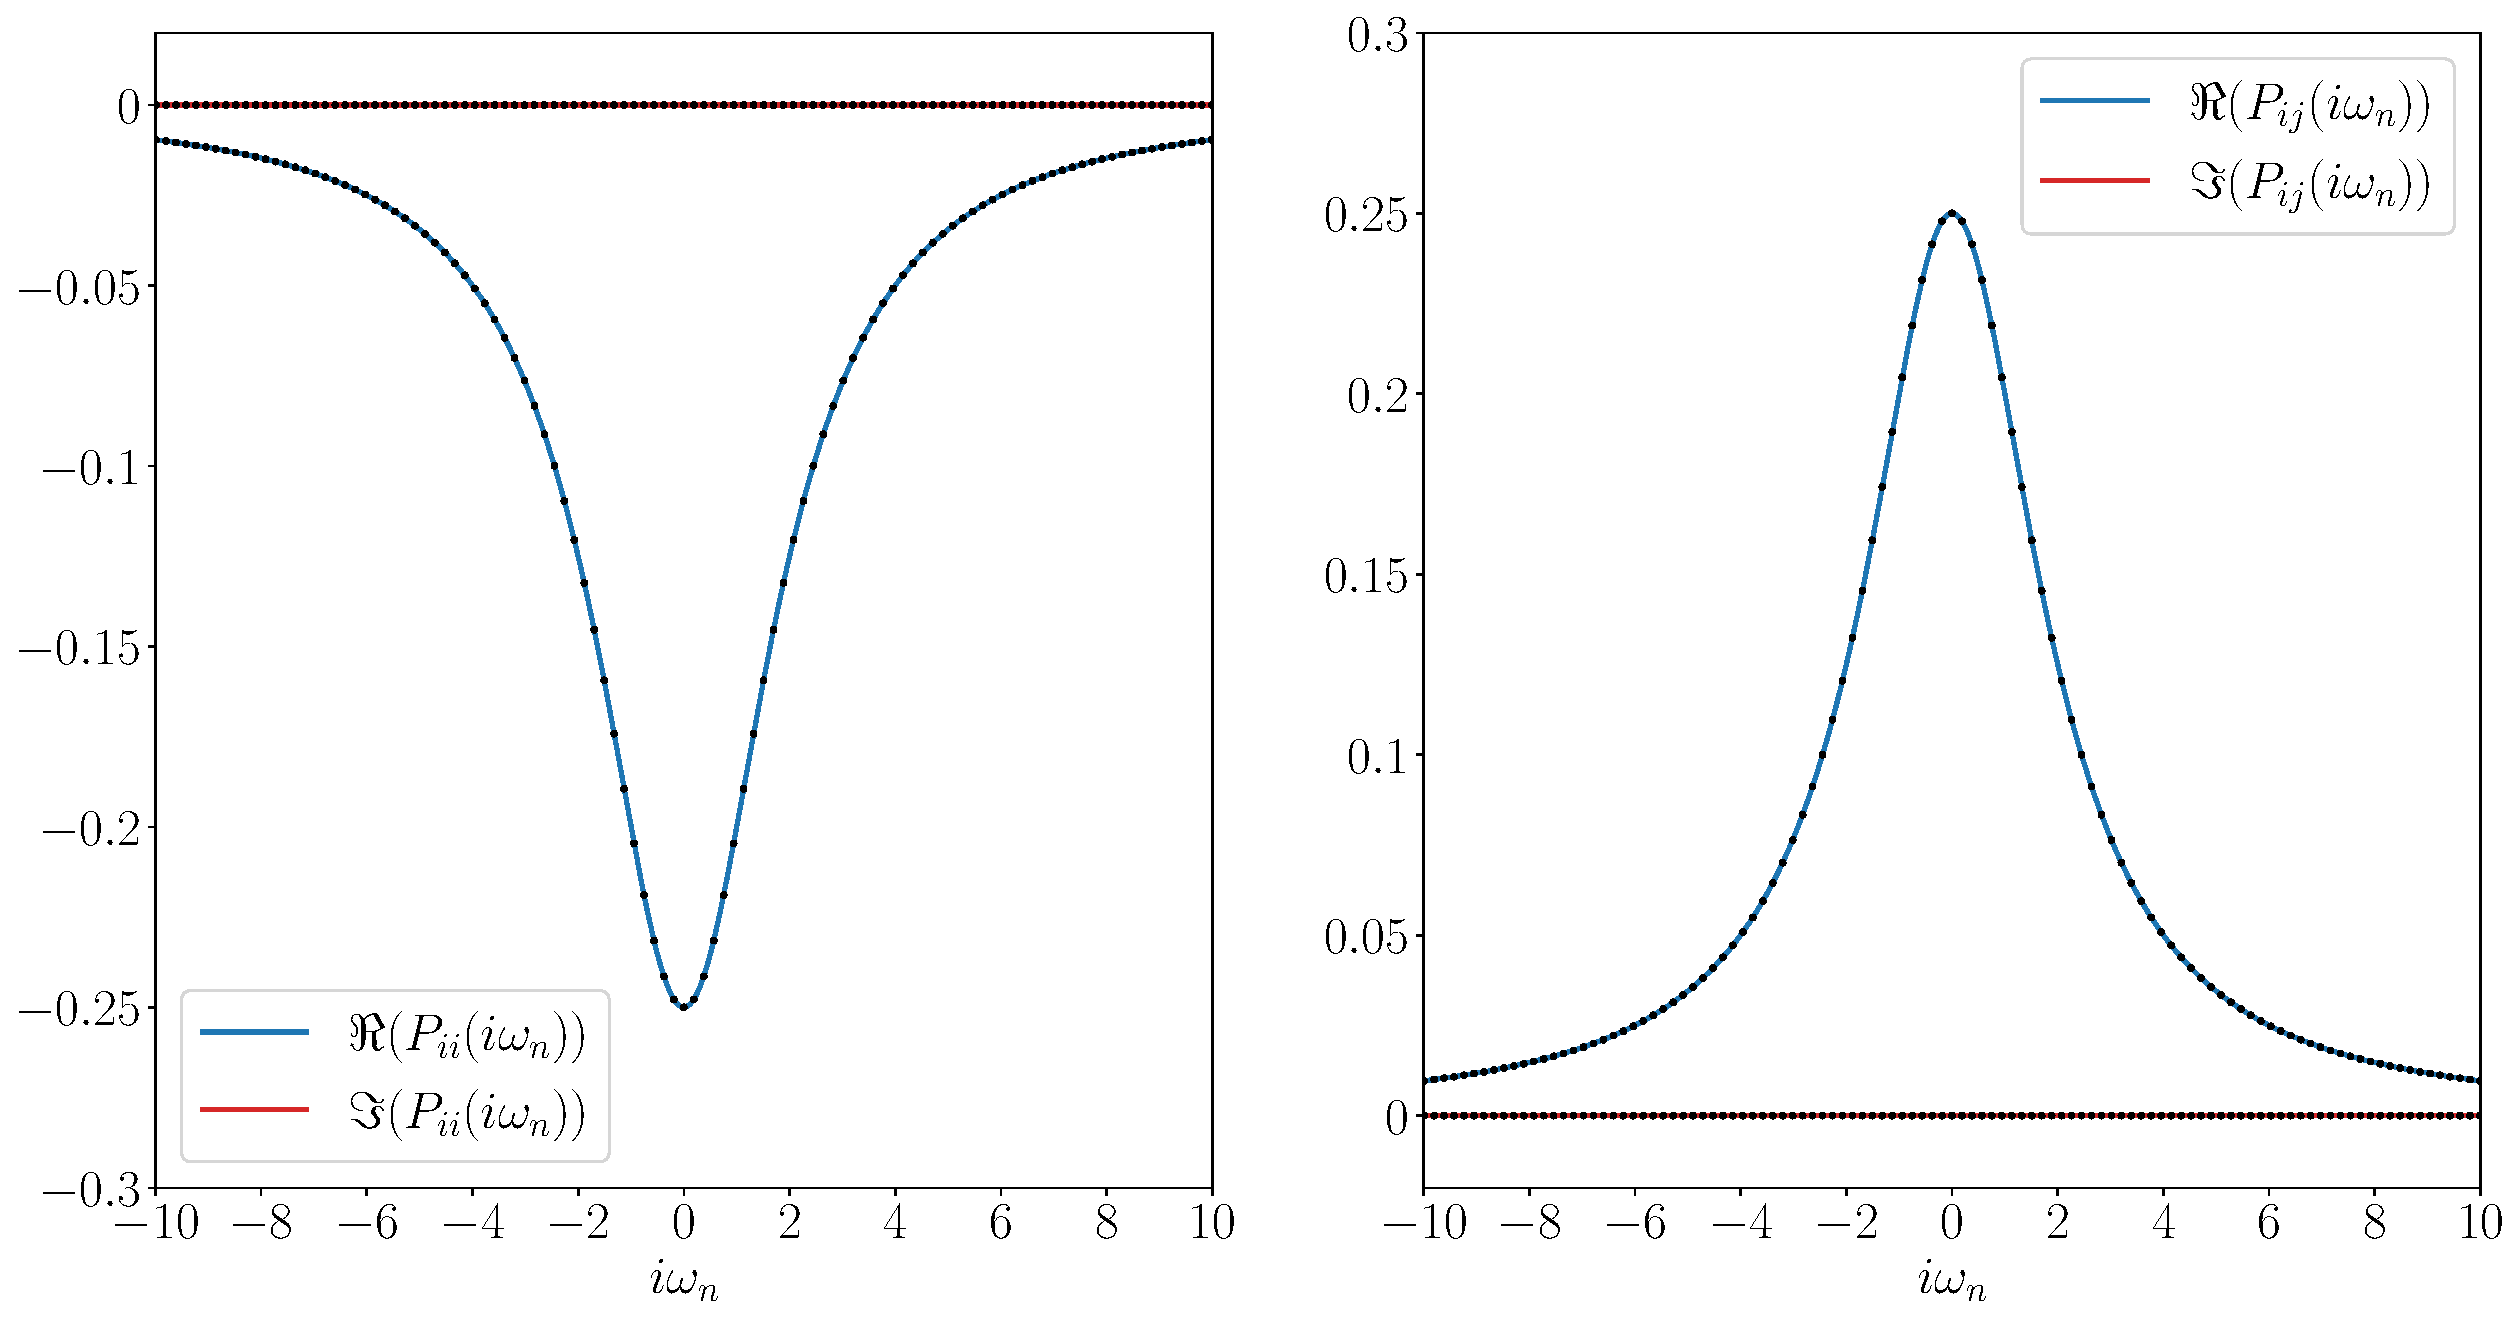
\includegraphics[scale=0.45]{P.pdf}
\end{figure}
\newpage
\noindent
\begin{equation}
W(i\omega_n)=(\mathbb{1}-v\cdot2P(i\omega_n))^{-1}\cdot v
\end{equation}
\begin{figure}[h!]
\center
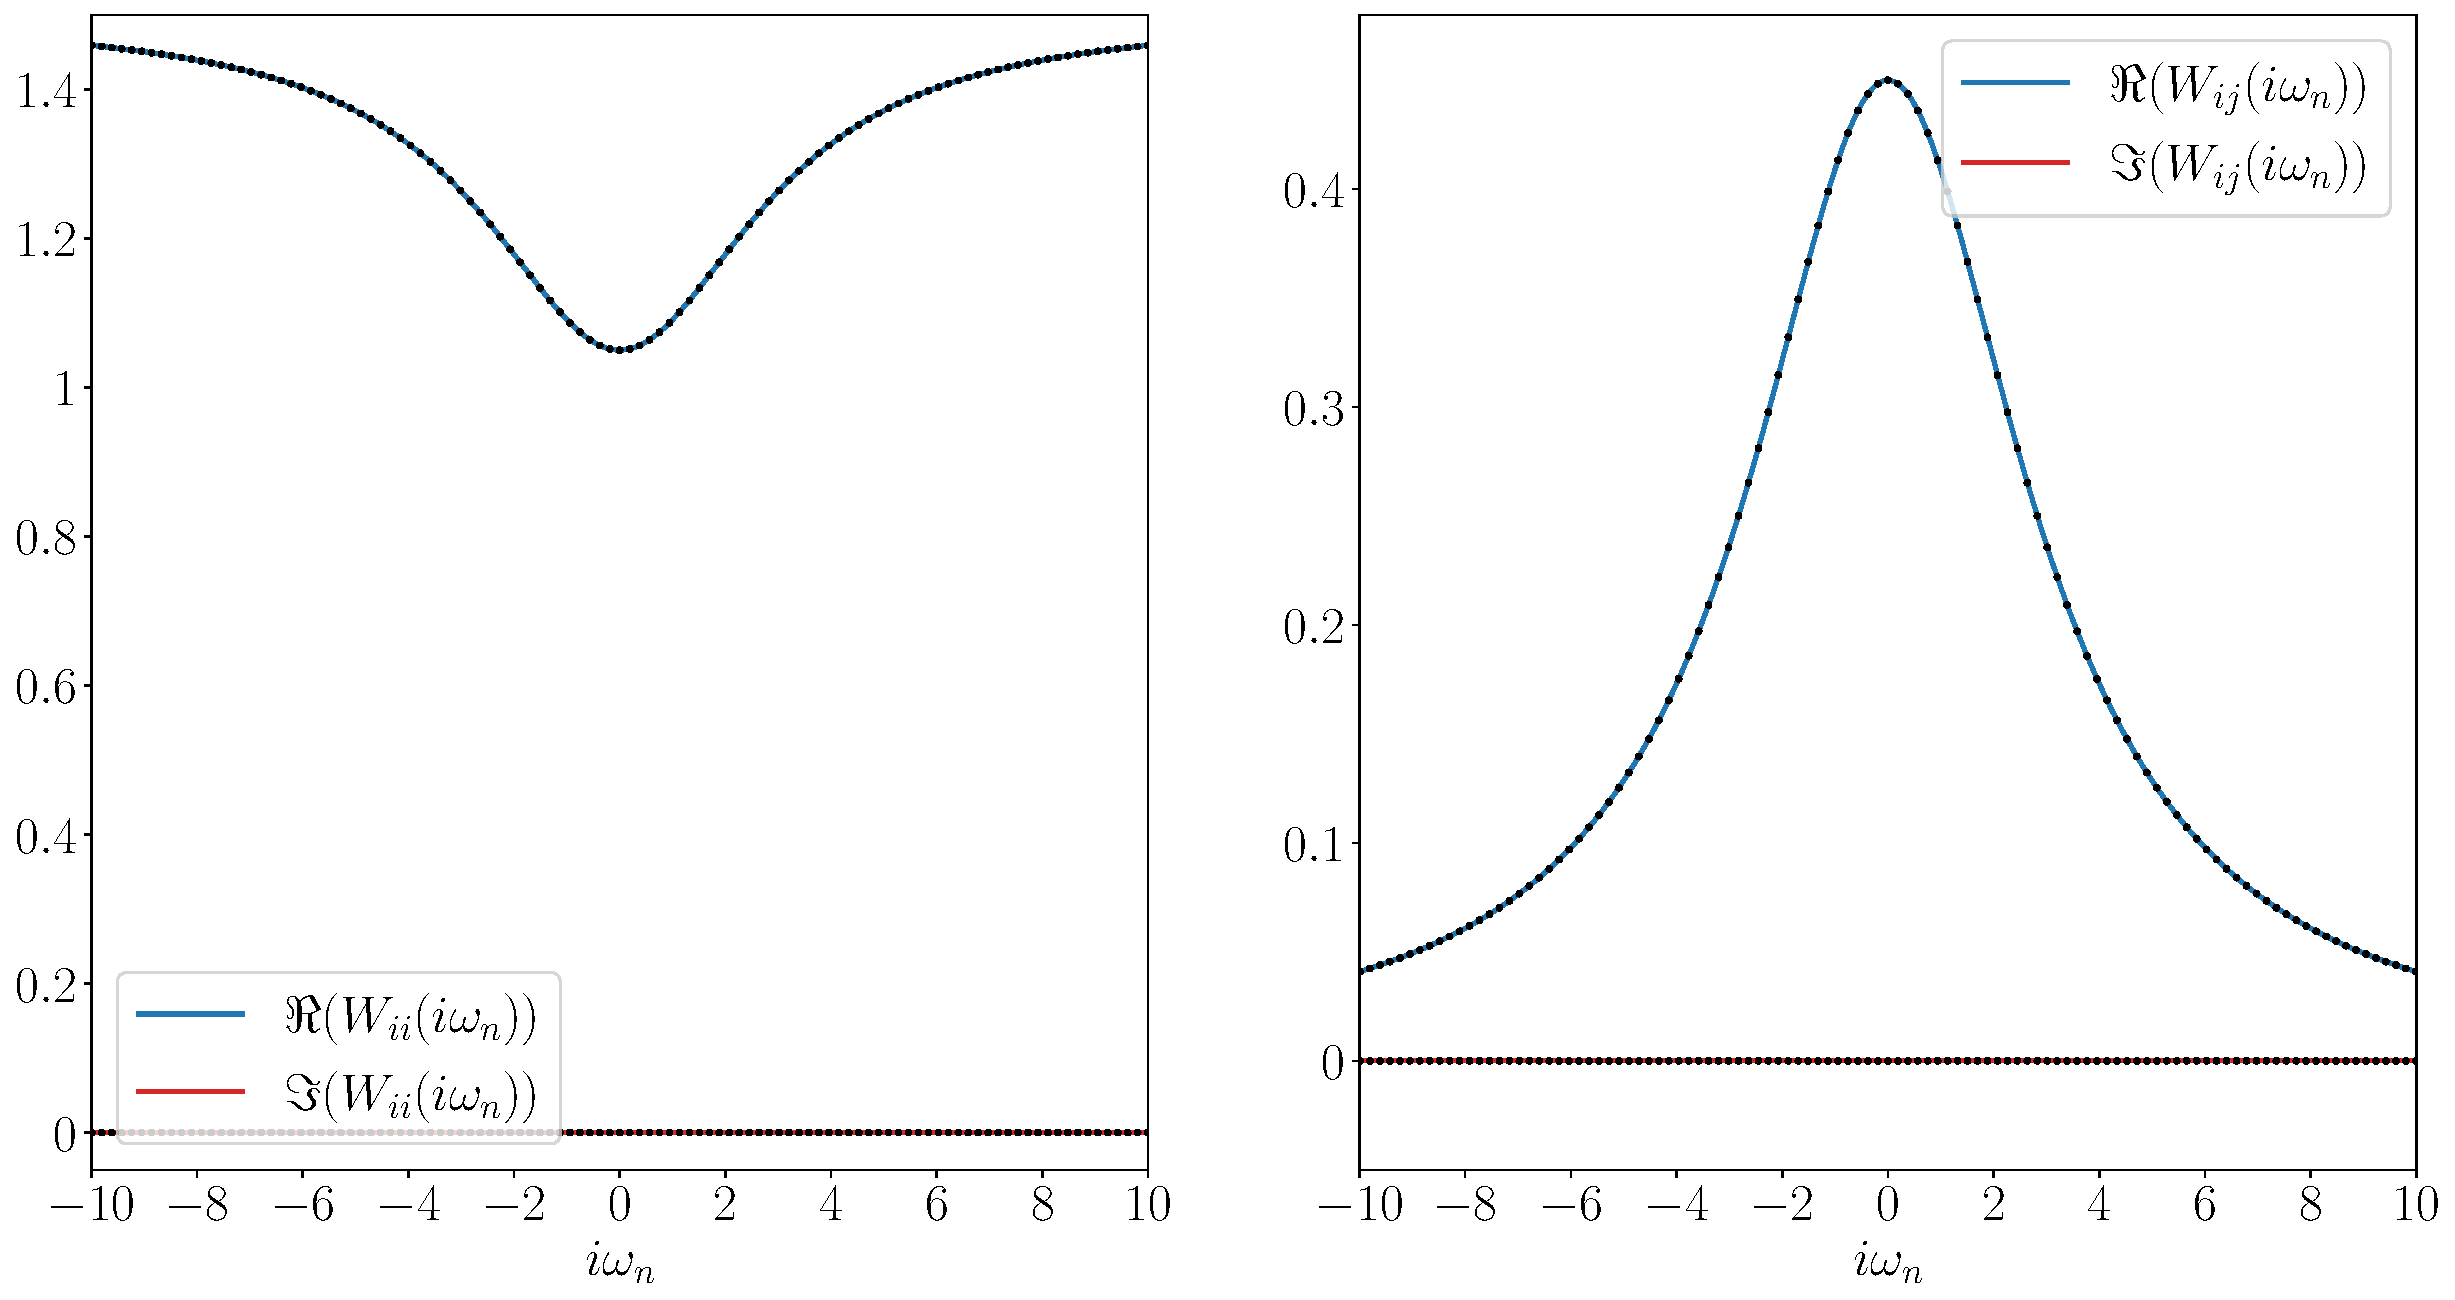
\includegraphics[scale=0.45]{W.pdf}
\end{figure}
\begin{equation}
\Sigma(\tau)=-G^0(\tau)W(\tau)
\end{equation}
\begin{figure}[h!]
\center
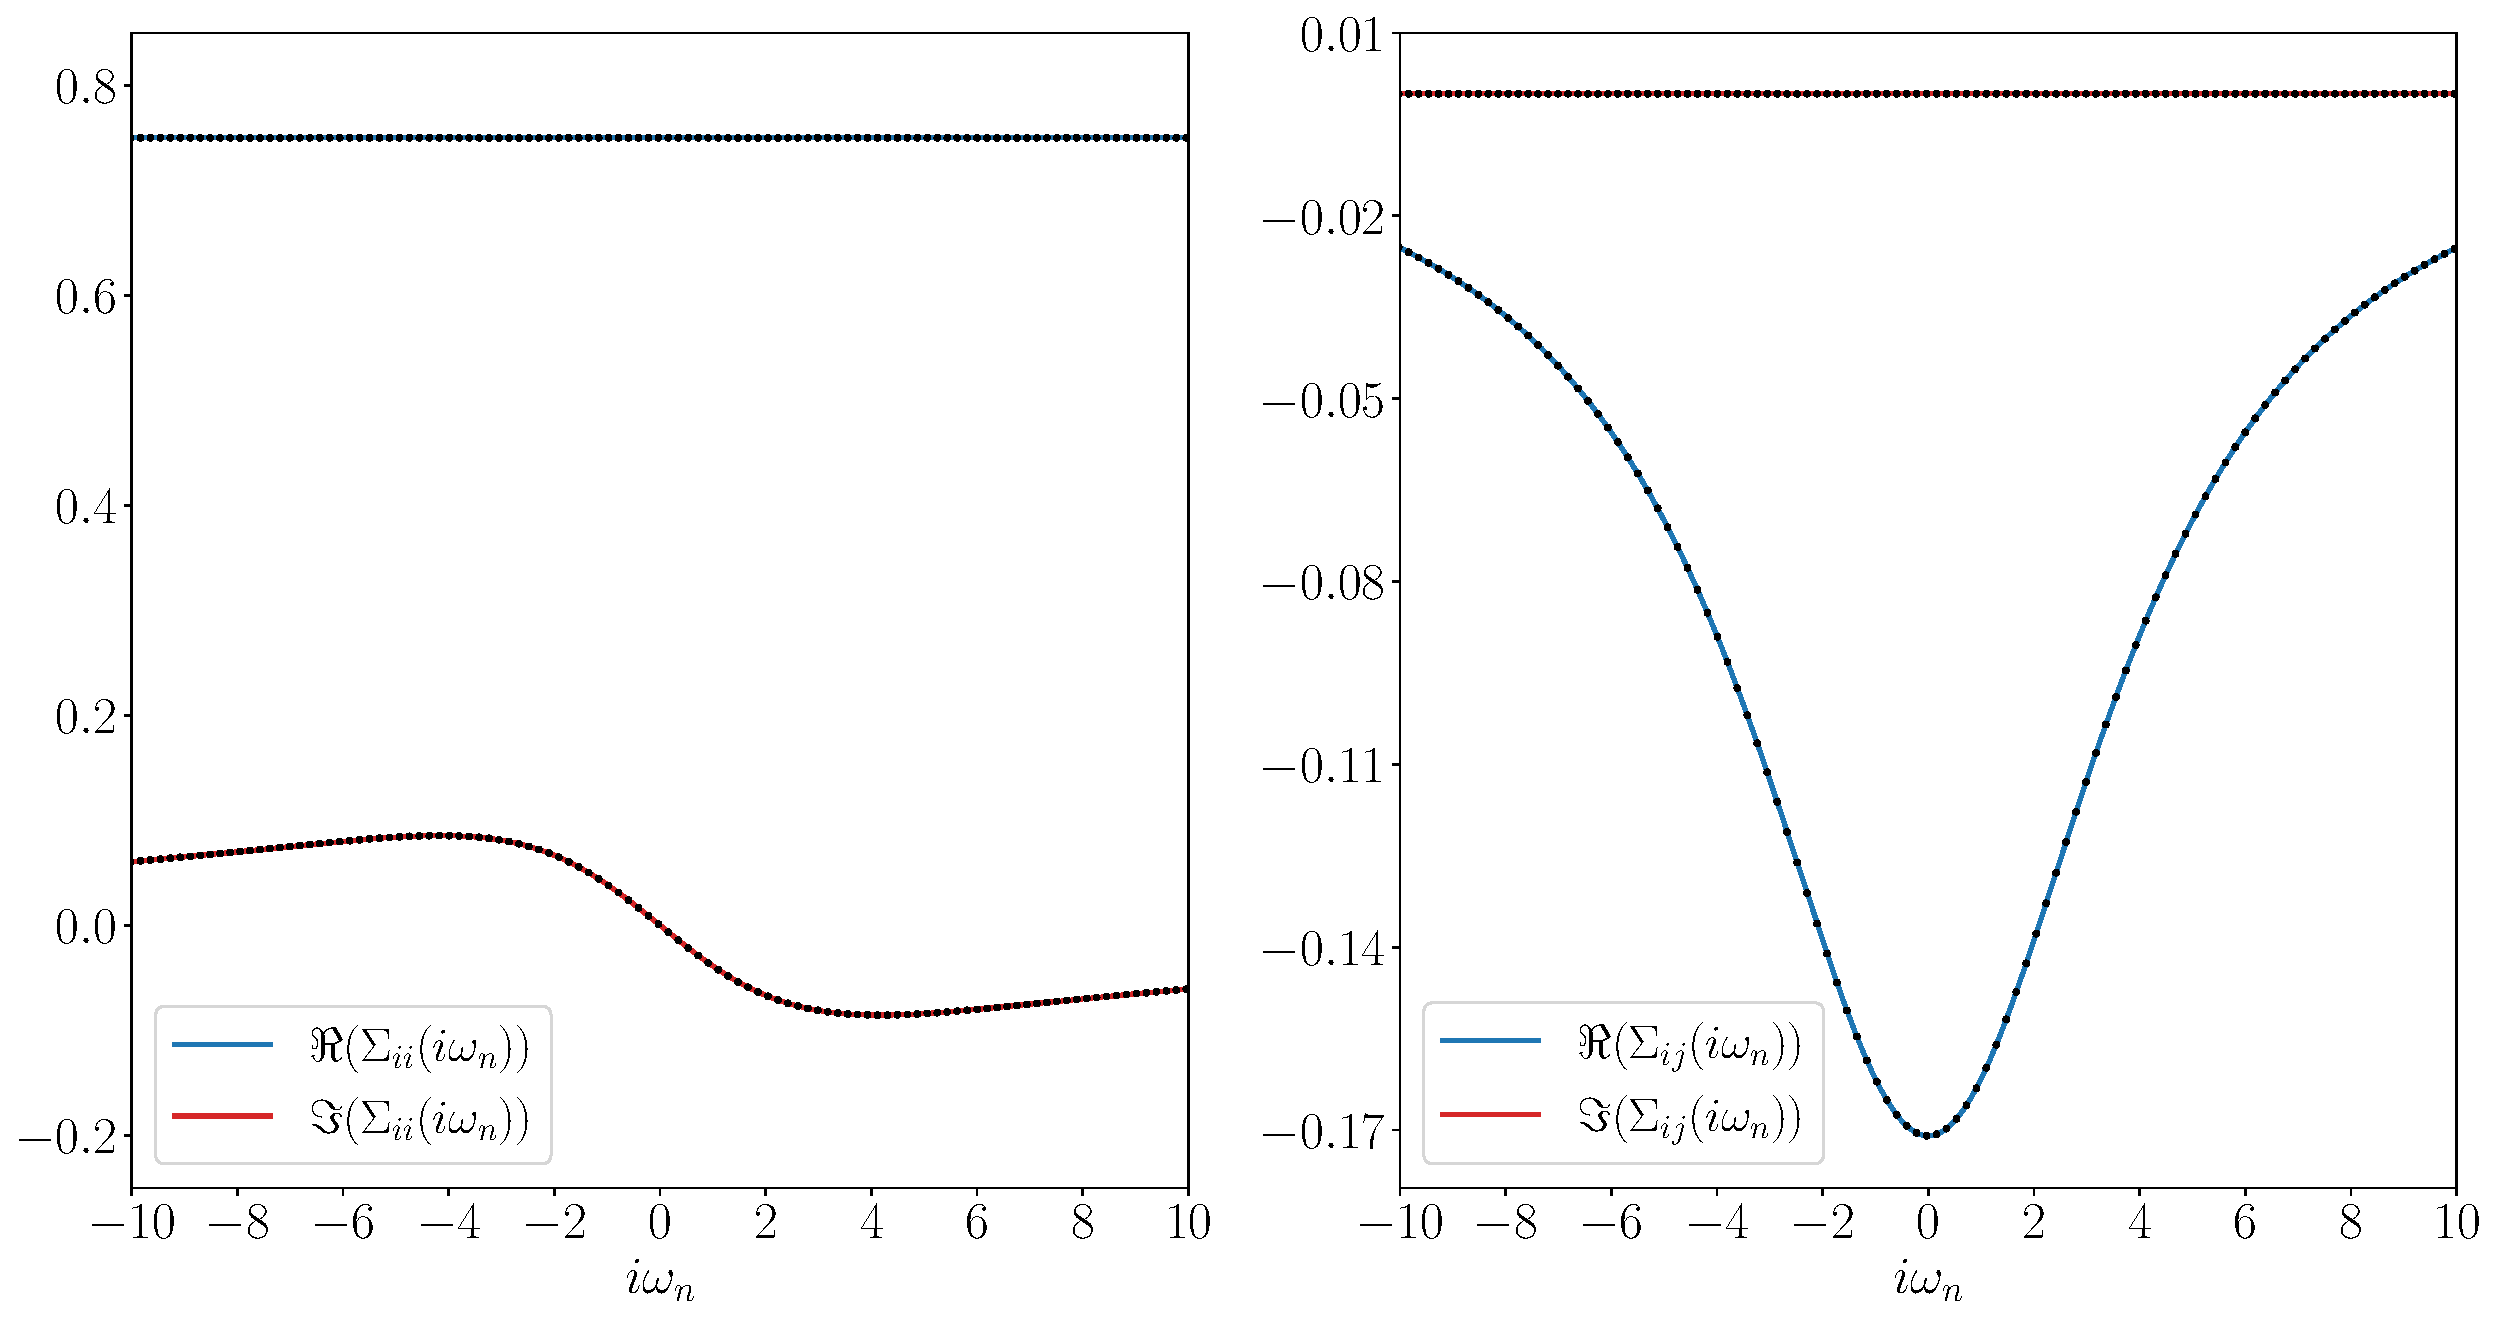
\includegraphics[scale=0.45]{S.pdf}
\end{figure}
\newpage
\noindent
\begin{equation}
G(i\omega_n)=((G^0)^{-1}(i\omega_n)-\Sigma(i\omega_n))^{-1}
\end{equation}
\begin{figure}[h!]
\center
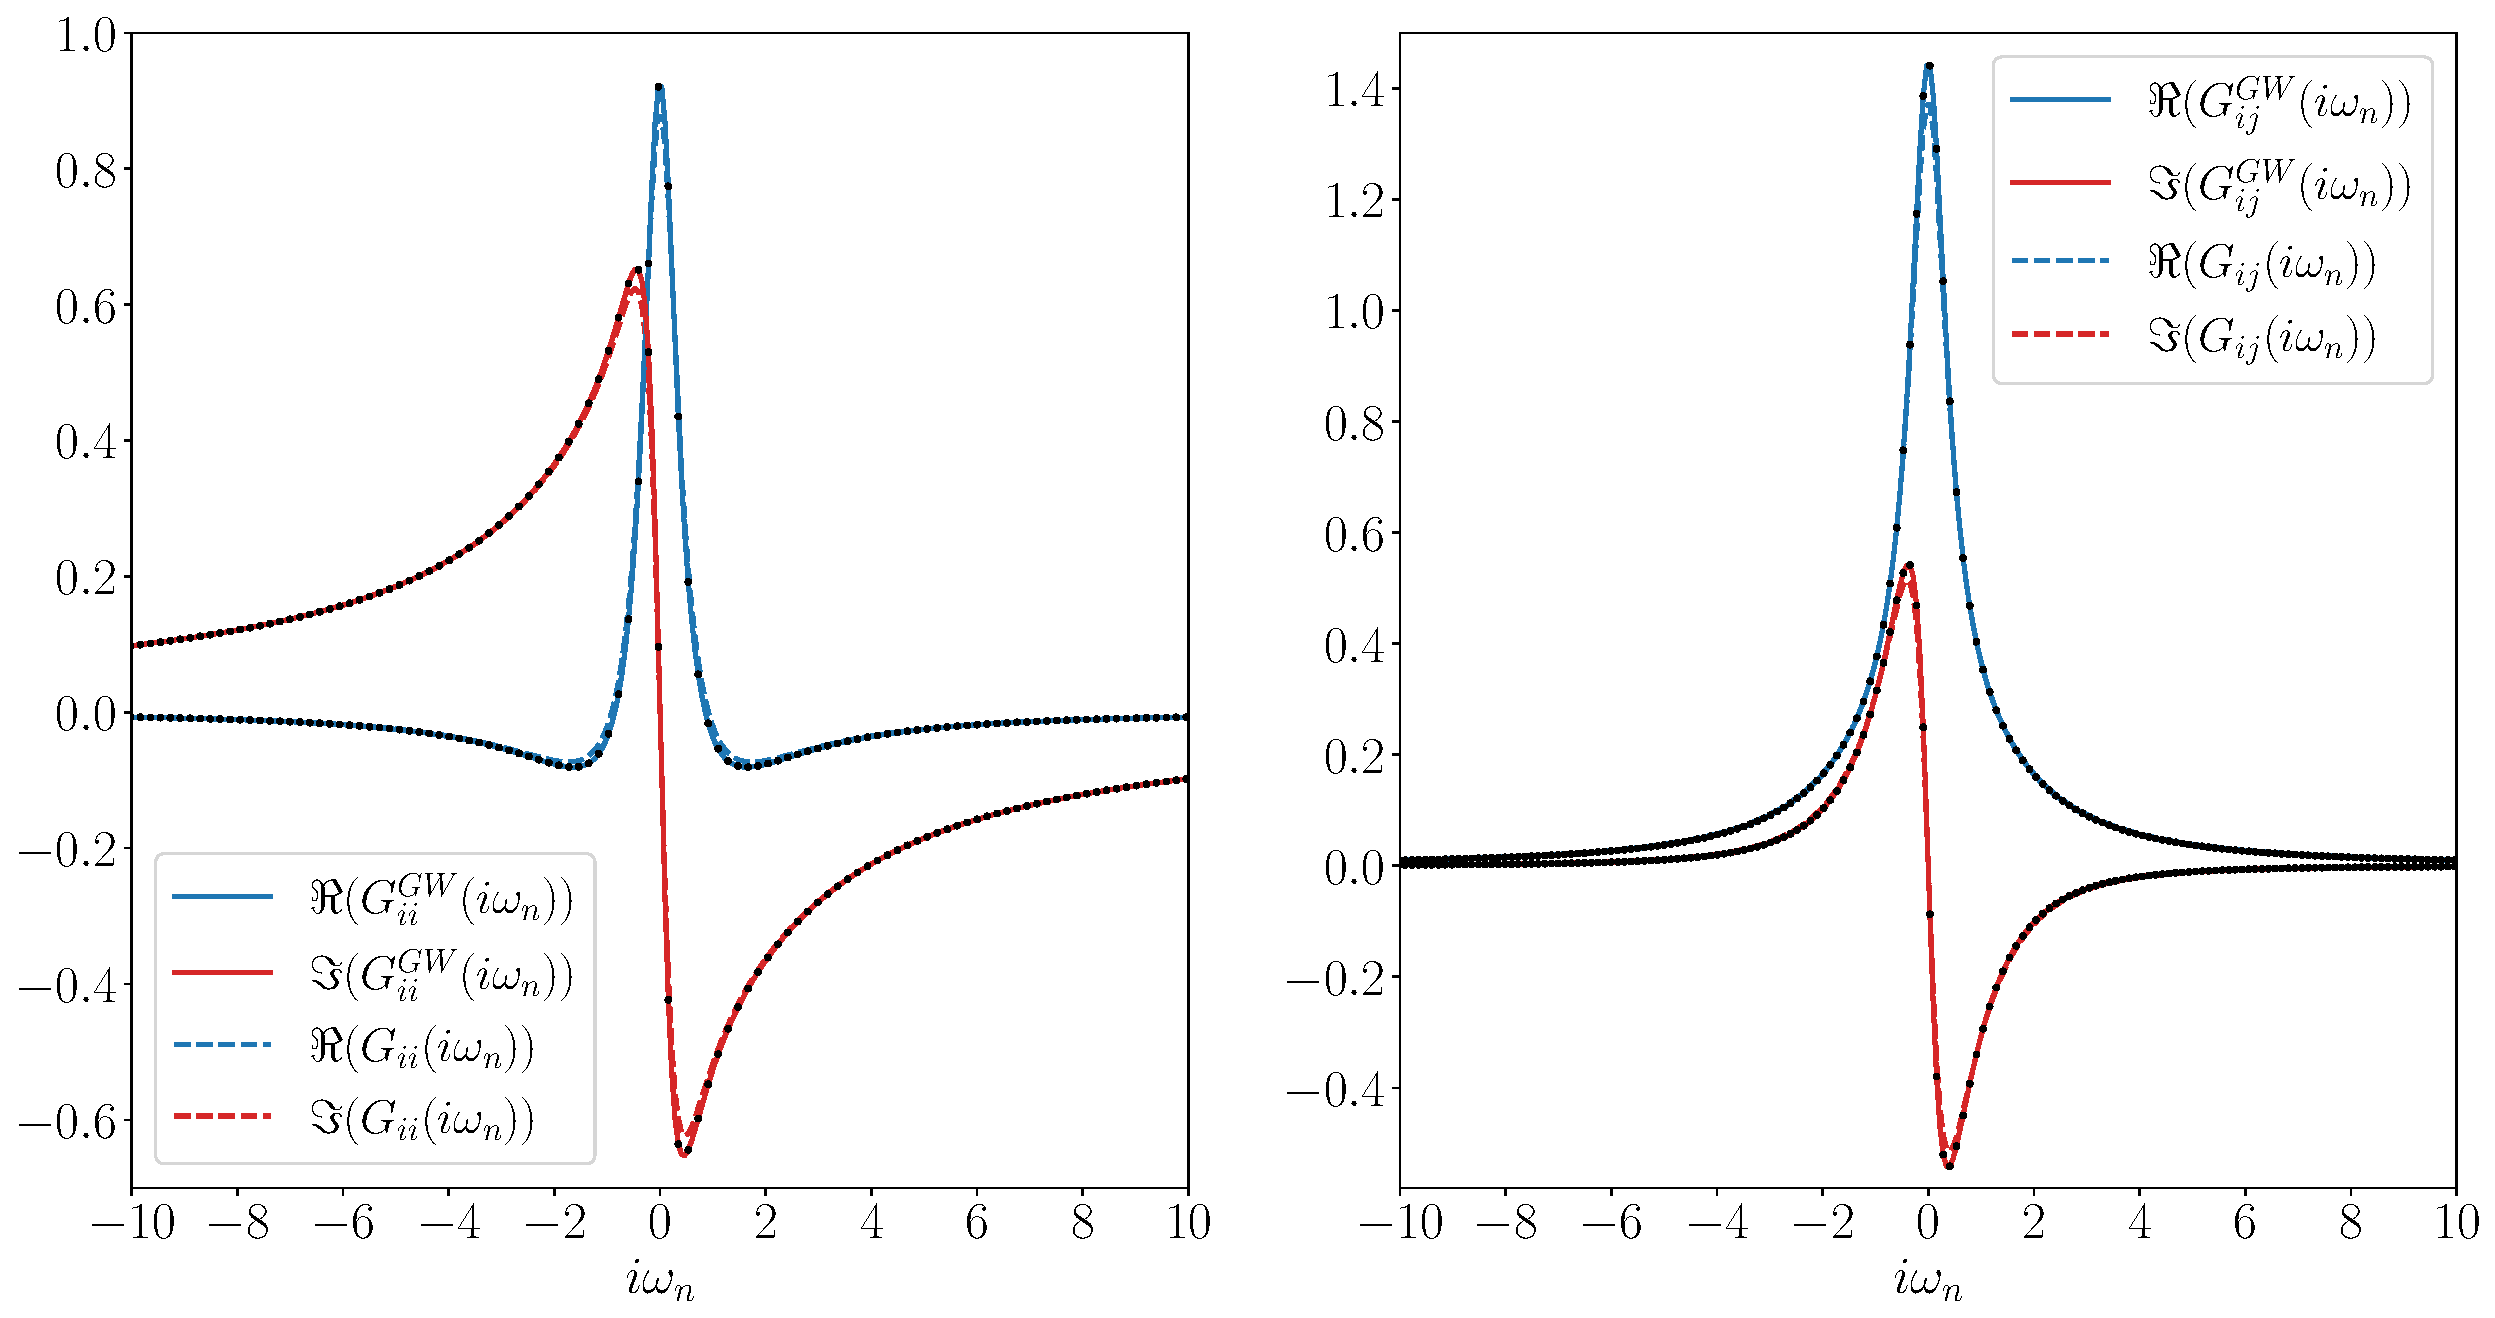
\includegraphics[scale=0.45]{G.pdf}
\end{figure}\\
Some notes on the implementation:
\begin{itemize}
	\item Coulomb potential is set as a diagonal matrix with $U$ on the diagonal
	\item Hatree potential is found by multiplying the Coulomb potential times the density of $G^0$
	\item As seen in the figure for $W$, the real diagonal part contains a shift which makes it not go to zero for large $|i\omega_n|$. This shift is subtracted manually to avoid problems with the Fourier transforms and finding the self-energy. This offset is equal to $U=1.5$ so I explicitly subtract $U$, if I just take the first diagonal element for $W$ on the first frequency point I get $1.4999564368347733+i3.9127207136660495\cdot 10^{-16}$ but using this value over $U$ will result in a slightly wrong self-energy, even if taken as real.
	\item The Hatree term is explicitly added when calculating $G$ to avoid unneeded Fourier transforms
	\item When using the exact shift of $U=1.5$ all the quantities pass the \texttt{np.allclose()} test but when the numerical shift is taken the self-energy fails this test. But when taking a much larger Matsubara frequency mesh this is no longer the case, as expected.
\end{itemize}



\end{document}